
\begin{figure}[t]

\centerline{
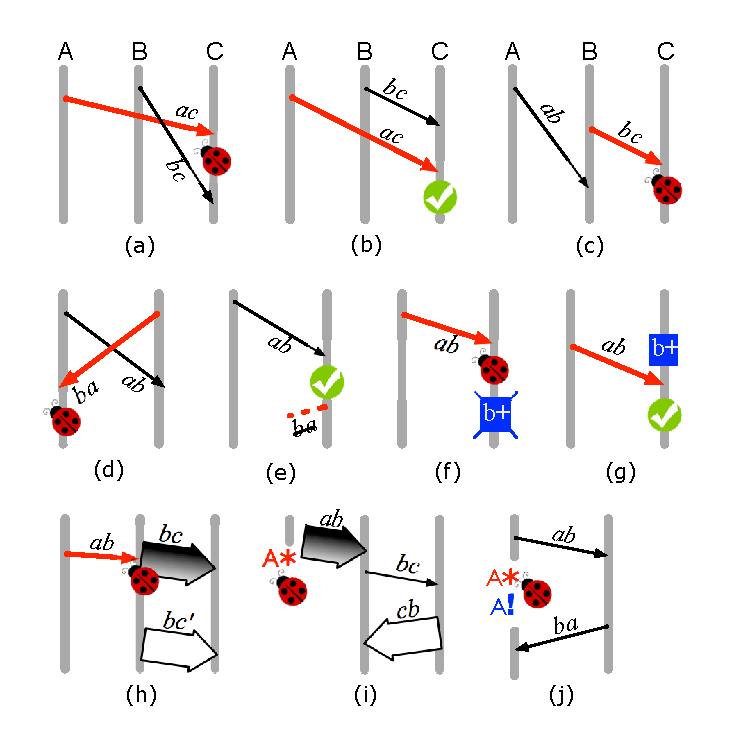
\includegraphics[width=3.5in]{F/patterns/basics.eps}
%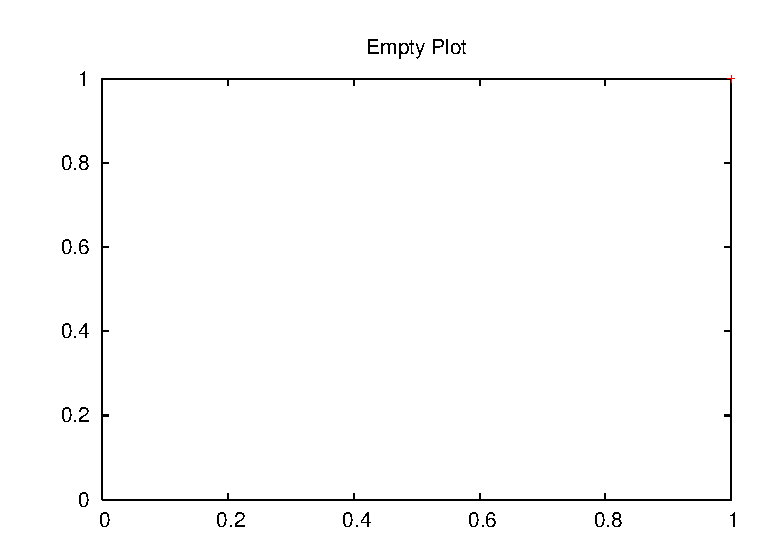
\includegraphics[width=0.5\textwidth]{F/empty.eps}
}
\vminten
\mycaption{pat}{Triggering patterns (\sec{\ref{trig-time}})}
{The three vertical lines represent the timeline of nodes A, B and C.
An arrow with \ts{xy} label implies a message from X to Y.  A square
box with label \ts{x+} implies a local state-modifying computation at
node X.  A thick arrow implies a set of messages performing an atomic
operation.  \ts{X*} and \ts{X!} implies a crash and reboot at node X
respectively (\sec\ref{met-pres}). All figures  are discussed in
\sec{\ref{trig-time}}}

\end{figure}



\if 0
\newtxt{The three lines represent
timeline of nodes A's, B's, and C's events (\ie\ sending/receiving
messages, local computations, crashes/reboots). Arrow lines ac mean
messages from A to C. Square boxes b+ mean local computations in B.
Thick arrows mean a set of messages doing an atomic operation. A*
means a crash of A, and A! means a reboot of A.  Figure (a)
illustrates an order violation pattern due to a race of two message
arrivals on node C (\ie\ messages ac/bc), which the bug would not
manifest if C receives the messages as in figure (b). Figures (c) and
(d) illustrate order violations between a message arrival and a
message sending (\ie\ ab/bc in (c), and ab/ba in (d)) which the bugs
would not happen if B receives the message ab before it sends a
message as in figure (e). Figure (f) illustrates an order violation
pattern between a message arrival and a local computation (\ie\ ab/b+)
which the bug would not manifest, if ab arrives after B has finished
b+ computation as in figure (g). Figure (h) illustrates an atomicity
violation that a message ab comes during B is doing an atomic
operation. Figure (i) illustrates a fault-timing pattern that A
crashes during an atomic operation (\ie\ A*/ab). Figure (j)
illustrates a reboot timing pattern that A crashes and reboots during
B processing a message ab, and A does not expect a message ba; the bug
would not happen if B tries to send ba and finds out A is dead. } }
\fi
